\begin{definefigure}{fig:compression}
\captionsetup[subfigure]{labelformat=empty}
\centering
\begin{subfigure}{0.4\columnwidth}
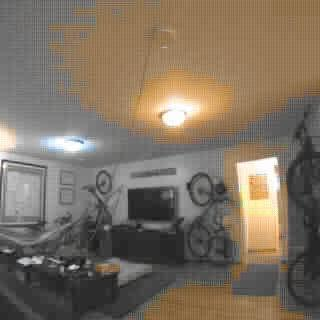
\includegraphics[width=\linewidth]{images/30.jpeg}
\vspace{-1.5\baselineskip}
\caption{30}
\label{fig:30}
\end{subfigure}
%
\begin{subfigure}{0.4\columnwidth}
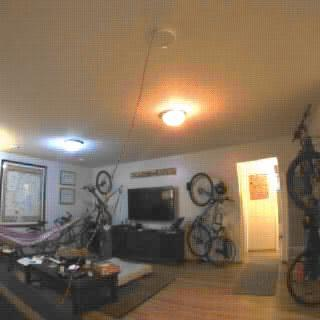
\includegraphics[width=\linewidth]{images/70.jpeg}
\vspace{-1.5\baselineskip}
\caption{70}
\label{fig:70}
\end{subfigure}
\par\medskip
\begin{subfigure}{0.4\columnwidth}
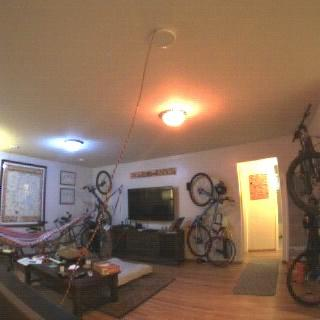
\includegraphics[width=\linewidth]{images/93.jpeg}
\vspace{-1.5\baselineskip}
\caption{93}
\label{fig:93}
\end{subfigure}
%
\begin{subfigure}{0.4\columnwidth}
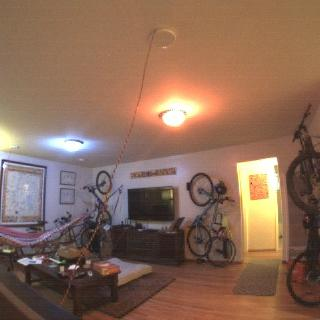
\includegraphics[width=\linewidth]{images/raw.jpeg}
\vspace{-1.5\baselineskip}
\caption{raw}
\label{fig:raw}
\end{subfigure}
\caption{An image compressed with different quality factors. \normalfont{In this scene, we set smart lights to bright, intense colors to elucidate the effects of compression on color representation. Compression is performed on the mosaiced version of the image, which after transmission is demosaiced into the color representations displayed. Due to this, an image compressed with a low quality factor loses significant color information compared to the raw image. Luckily, high quality factors produce a near-indistinguishable representation of the raw image. We explore a more quantitative view of image similarity in \cref{fig:ssim}.}}
\end{definefigure}

\begin{definefigure}{fig:size-time-energy}
    \centering
    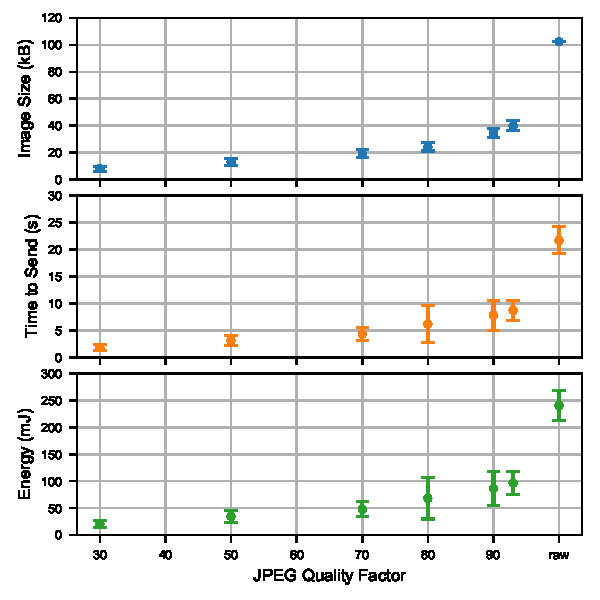
\includegraphics[width=\columnwidth]{figs/size_time_energy.pdf}
    \caption{Effects of JPEG compression on image size, time to send, and energy to send.
        \normalfont{
            Compression provides exponential decrease in image size, which directly relates to decreases in the time and energy required to send images. Using a low quality factor results in images that are 8.2\% the size of the original raw image. The amount of time and energy required to send images exhibit more variance than image size. This is the result of occasional packet loss and backoff during image transmission. Larger images require more packets and thus a higher probability of this occurring.
        }}
\end{definefigure}

\begin{definefigure}{fig:ssim}
    \centering
    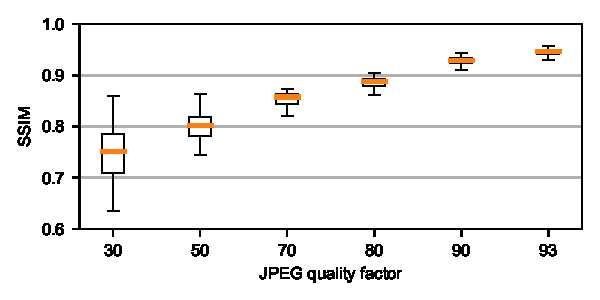
\includegraphics[width=\columnwidth]{figs/jpeg_ssim.pdf}
    \caption{\normalfont{The image structural similarity index (SSIM) of images compressed at various JPEG quality factors.
        A higher SSIM indicates that an image is a closer representation to the original raw image.
        While a low quality factor results in smaller compressed images, it results in a significant loss in image structural similarity. Quality factors 90 and 93 provide a >90 SSIM, suggesting that they are near identical representations of the original image.
    }}
\end{definefigure}

\begin{definefigure*}{fig:lifetime}
\centering
\begin{subfigure}{0.445\textwidth}
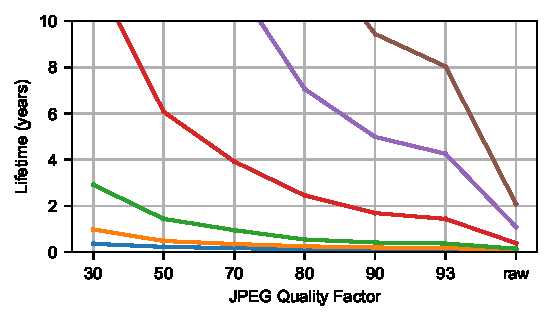
\includegraphics[width=\linewidth]{figs/lifetime_periodic.pdf}
\label{fig:lifetime_periodic}
\vspace{-1.5\baselineskip}
\caption{Periodic}
\end{subfigure}
%
\begin{subfigure}{0.545\textwidth}
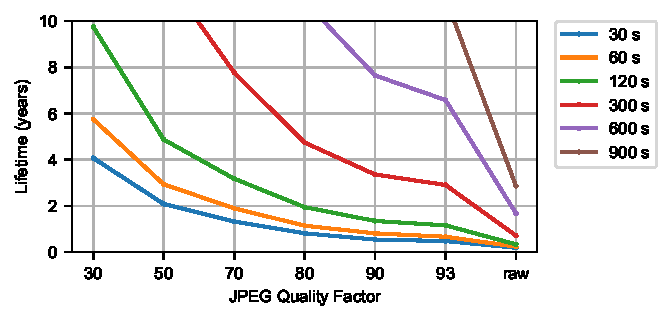
\includegraphics[width=\linewidth]{figs/lifetime_event_60.pdf}
\label{fig:lifetime_event}
\vspace{-1.5\baselineskip}
\caption{Reactive}
\end{subfigure}
\vspace{-1\baselineskip}
\caption{\normalfont{
    Estimated lifetime from a numerical model. Two workloads are simulated: periodic and reactive. A periodic workload takes a picture at a fixed interval, while the reactive workload models motion events captured by a PIR sensor. We vary the quality factor of images sent, which has a direct impact on the lifetime of the workloads. Each colored line represents a different period of the periodic workload, or the duration of the back off after an event for the reactive workload. As expected, the reactive workload results in a longer lifetime as it captures and transmits fewer images in times of less activity like nighttime. For both workloads, \name is able to transmit images compressed at quality 90 and still achieve a one to five year lifetime based on period or back off duration.
}}
\end{definefigure*}

\begin{definefigure}{fig:multiple}
    \centering
    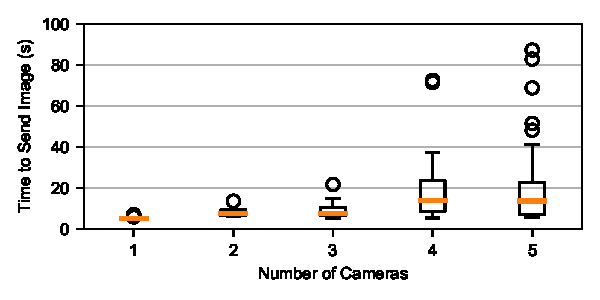
\includegraphics[width=\columnwidth]{figs/multiple_cameras.pdf}
    \vspace{-2\baselineskip}
    \caption{\normalfont{An image's time to send as number of \names on the network increases. All sensors are within one meter radius of each other, and configured to capture and transmit images on motion events to generate the worst case collision condition. Images are compressed with quality 90.
    }}
\end{definefigure}

\begin{definefigure}{fig:map}
    \centering
    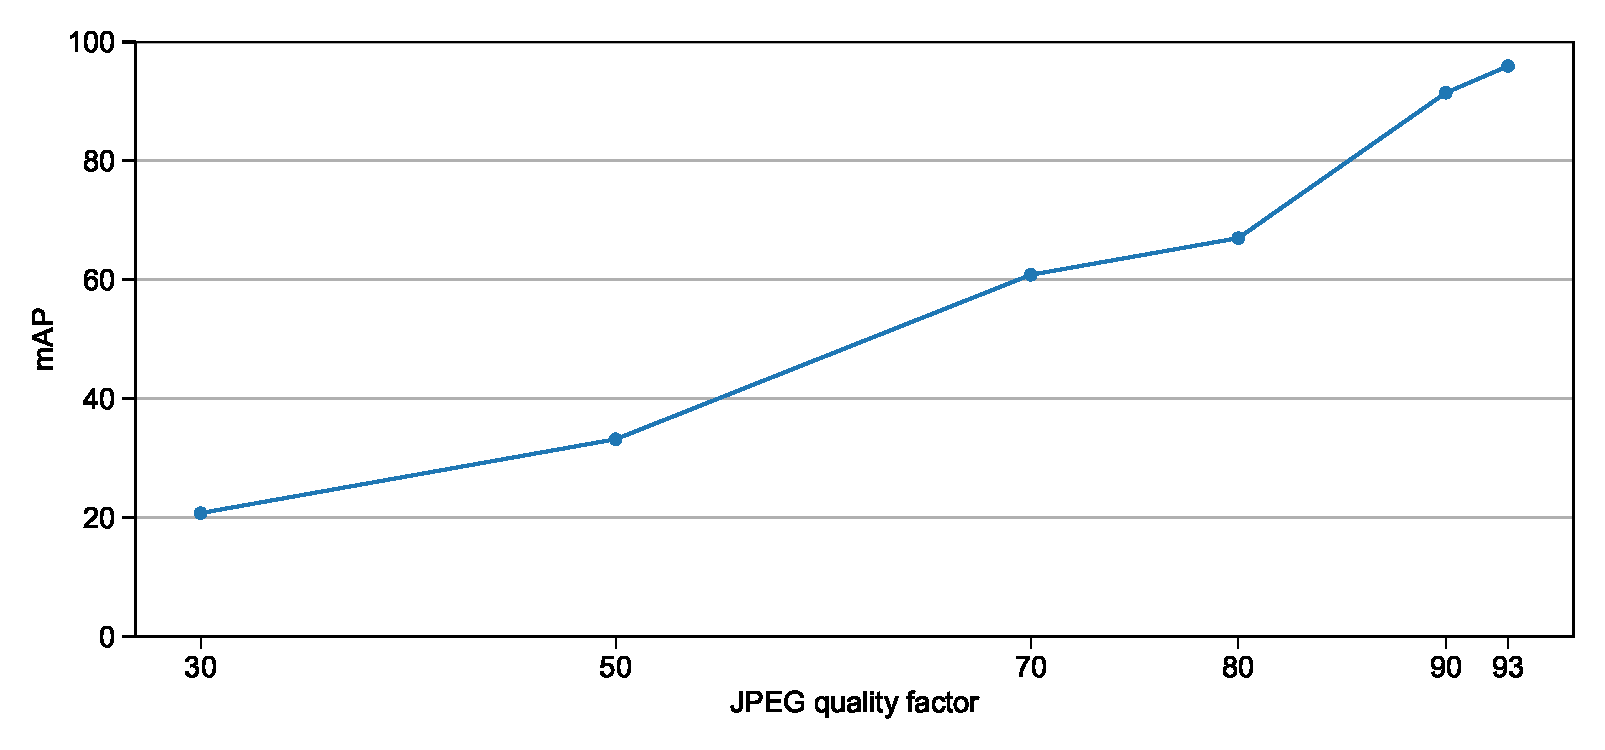
\includegraphics[width=\columnwidth]{figs/jpeg_mAP.pdf}
    \vspace{-2\baselineskip}
    \caption{\normalfont{Mean Average Precision (mAP) of YOLOv3 person detection on compressed images compared to original raw versions. An IoU of 0.5 is used. Based on the qualitative and quantitative results of image similarity from \cref{fig:compression} and \cref{fig:ssim} it is surprising that mAP degrades so quickly as the compression quality factor decreases. A quality factor of 90 or higher is necessary to achieve the near the same detection performance as a raw image}}
\end{definefigure}

\begin{definefigure}{fig:distance}
    \centering
    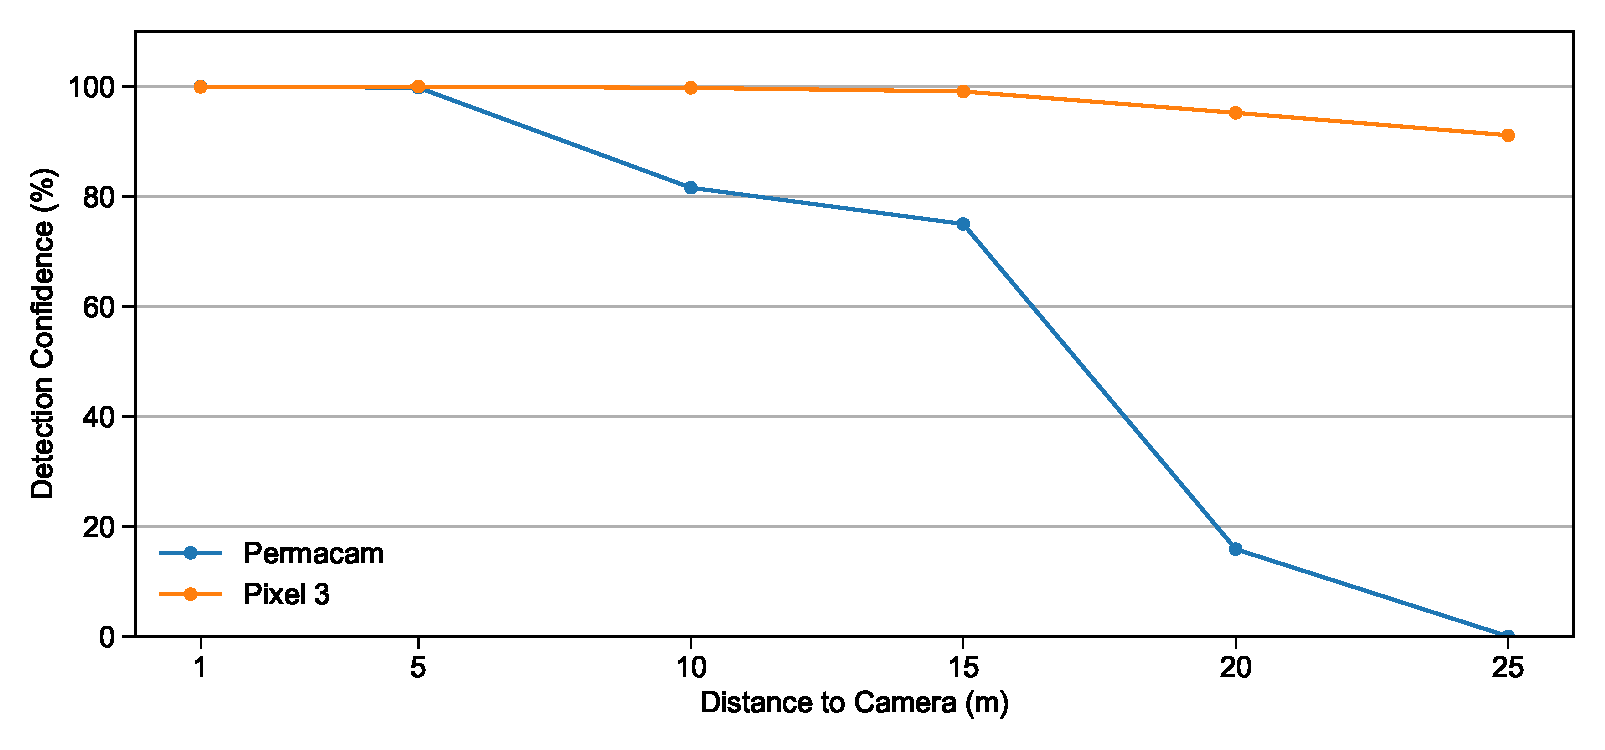
\includegraphics[width=\columnwidth]{figs/distance_detection.pdf}
    \caption{\normalfont{
        Detection confidence as distance from camera to person is increased. Compared to a modern smartphone camera, the camera on \name can not compete due to limited resolution. However, images captured by \name still enable person detection at a distance of 15-20 meters. This distance is generally sufficient for most indoor spaces.
    }}
\end{definefigure}

\begin{definetable}{tab:local-inference}
\setlength\tymin{30pt}
\footnotesize
\begin{tabulary}{\columnwidth}{LCCCCC}
Dimension (pixels) & Latency\newline(s) & MOPs & Energy\newline(mJ) & Memory (kB) & Accuracy (\%) \\
\hline
48 & 1.72 & 0.450 & 17.2 & 73.7 & 68.6 \\
72 & 2.71 & 1.01 & 27.0 & 91.0 & 69.2 \\
96 & 3.64 & 1.80 & 36.4 & 115. & 72.4 \\
120 & 5.10 & 2.81 & 50.9 & 146. & 74.7 \\
\end{tabulary}
\caption {\normalfont{
    Latency, millions of operations, energy, peak memory, and accuracy 
    of local person classification. Images must be downscaled from full resolution, as inference on a 320x320 image requires too much runtime memory. The quantized version of model weights are used to measure accuracy of the validation set. The highest accuracy achieved is only 74.7\%, and requires 5.1 seconds of continuous computation.
}}
\end{definetable}

\begin{definetable}{tab:end-to-end}
\setlength\tymin{1cm}
\small
\begin{tabulary}{\columnwidth}{LCCC}
Compression\newline Quality & Size\newline(kB) & Latency\newline(s) & Energy\newline(mJ) \\
\hline
30  & 1.98 & 0.513 & 4.23\\
50  & 3.25 & 0.764 & 6.95\\
70  & 4.82 & 1.12 & 10.3\\
80  & 6.19 & 1.31 & 13.2\\
90  & 9.12 & 1.86 & 19.5\\
93  & 10.6 & 2.13 & 22.7\\
raw & 25.6 & 4.91 & 54.7\\
\end{tabulary}
\caption {\normalfont{Time and energy required to send 160x160 images end-to-end. Images are compressed with varying JPEG qualities. Sending compressed images requires less time and energy than performing person classification on lower resolution images.}}
\end{definetable}

\begin{definefigure}{fig:cycle-per-byte}
    \centering
    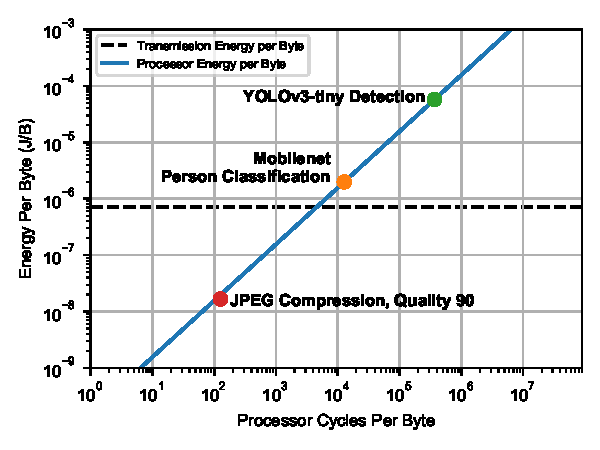
\includegraphics[width=\columnwidth]{figs/cycles_per_byte.pdf}
    \caption{The required energy per byte of image data to run different algorithms on the processor used by \name{}.
        \normalfont{
            The slope of the solid line represents the energy per cycle of the processor. The dashed line represents the energy per byte of a compressed transmission of an image. Three algorithms are plotted here: JPEG compression with quality factor 90, our custom MobileNets v1 person classifier, YOLOv3-tiny object detection. We estimate the cycles and energy required of YOLOv3, as it requires more memory than available on our microcontroller.
        }}
\end{definefigure} 

\begin{definetable}{tab:measurements}
\setlength\tymin{1cm}
\begin{tabularx}{LS[table-format=1.3]S[table-format=2.2]}
{Operation} & {Latency (s)} & {Energy (mJ)} \\
\hline
Image Capture           & 1.10  & 4.96\\
JPEG Compression (Q=90) & 0.203 & 1.71\\
Image Transmission      & 6.67  & 73.8\\
\hline
Total                   & 7.973 & 80.47
\end{tabularx}
\caption {
    Latency and energy measurements for key operations on \name, including image capture, compression, and image transmission. Measurements are averaged over 20 images. %An image capture actually consists of multiple frames to calibrate the exposure. We configure \name to wait four frames before capturing an image.
}
\end{definetable}

\section{Evaluation}
We evaluate \name{} on our goals of deployability and capability through a number of experiments. We begin with an analysis of the effects of JPEG compression on image size, time to send, and energy. From this analysis, we use these measured metrics to estimate platform lifetime using different representative workloads. 
%We estimate platform lifetime using different configurations of workloads and image compression. 
We explore the capability of the platform by writing an object detection application on top of the \name{} end-to-end image transfer architecture. We evaluate the ability to detect objects in images captured by \name{} at varying qualities of compression and distance from the camera. We also implement local image inference in the form of person classification. We evaluate the performance of local classification, and compare it to image transmission.
%into the options for reducing energy spent transmitting images, including image compression and downsampling. We analyze the effects of these techniques have on resulting image quality. Based on the efficacy of image compression, we estimate lifetime using a simulation of \name{} to evaluate the longevity of the platform. We evaluate the capability of the platform by performing object detection tasks on the images that it captures. We measure the effects of design decisions on the accuracy of detections.  

\subsection{Image Compression}
\label{eval:compression}
A raw, full frame image from \name{}'s camera is over 100\,kB in size. Sending these raw images requires a significant amount of time and energy. We employ JPEG compression to significantly reduce image size. This decrease in size comes at the cost of reduced image fidelity and color representation.

We use the Moodstocks JPEC encoder to compress captured images in JPEG format. JPEC is a monochrome JPEG encoder, and we have configured \name{} to use the color version of the HM01B0 image sensor. The images captured are a "mosaiced" color filter array, and performing monochrome JPEG compression on a mosaiced image reduces color representation in addition to image fidelity. JPEG can be configured with different quality factors from 1 to 100. A lower quality factor results in a less accurate representation and smaller compressed size. Image size relates linearly to the time and energy required to send images. 
We configure \name to capture images, compress them with 6 different JPEG quality factors and transmit them. We collect 60 images, each with 6 compressed versions, and analyze the effect of compression on image size, time to send, and energy to send.
The results are displayed in \cref{fig:size-time-energy}. 

JPEG image compression allows an exponential decrease in image size with respect to the quality factor.
Compressing images at a high quality factor (JPEC's default 93) results in greater than a 2x reduction in image size, time to send, and energy required. There are diminishing gains after the knee of the curve at quality 90, but an image compressed with quality 30 is only 8\% the size of a raw image, on average. Image compression on mosaiced images from \name also does not appear to degrade the perceived quality of the image. We display four compressed and raw versions of the same image in \cref{fig:compression}. Qualitatively, and from a distance, these images appear nearly identical. However, closer inspection reveals artifacts and a significant loss in color fidelity with lower compression quality factors. Quality 93 and a raw image are nearly identical, while quality 30 is more obviously a lower quality compression. However, the important details in the image are preserved and still visible to the human eye.

To more quantitatively analyze the effects of compression on mosaiced images, we measure the Structural Similarity Index (SSIM)~\cite{wang2004image} of all 360 compressed images compared to their raw counterparts. SSIM is often used to measure the quality degradation of images due to compression or transmission. The results are summarized in \cref{fig:ssim}. A higher SSIM indicates that an image is a closer representation to the original raw image.
Even with a low quality factor of 30 or 50, the SSIM for images average above 0.75. With an image compressed with a high quality factor, the perceived similarity is above 0.9 and, as seen in \cref{fig:compression}, is almost indistinguishable from the raw image. These results suggest that using a quality factor of 90 or above on to compress images on \name is advantageous if we can afford the energy to send them.

\subsection{Lifetime}
\name is designed with the goal of a multi-year lifetime. While we are unable to physically measure the lifetime of the system, we can utilize a numerical model of the device to estimate lifetime. We utilize the model proposed by the authors of Permamote~\cite{jackson2019capacity} to estimate \name's lifetime. 
This simulator is designed to model the behavior of wireless energy harvesting sensors with common workloads like periodic and reactive sensing. The model is perameterized by various system characteristics, including regulator, harvester, and solar panel efficiency, energy storage characteristics and size, and various workload types.
This model operates a second-by-second calculation of incoming harvested energy and energy used by the device.
This simulator outputs a trace of state of charge over time, which can be used to estimate system lifetime.

We use this numerical model to estimate the lifetime of \name using two different workloads: periodic, and reactive. Periodic represents a workload where \name takes photos on a fixed interval, while reactive assumes that \name uses a PIR sensor to drive image capture. For reactive,
we model events as a Poisson distribution for each hour, with the busiest hour having an average event every minute. This is chosen to simulate a busy office setting. We vary the period of the periodic workload, and the backoff time after an event for the reactive workload.
Based on the measurements of the previous section, we also estimate lifetime when sending images of varying JPEG qualities.

We use the EnHANTs indoor irradiance dataset as input to our simulated energy harvester. We use the "SetupD" trace, which represents an average 100\,\uW/cm\textsuperscript{2} over the course of a year~\cite{Gorlatova_Infocom2011}. This irradiance is characteristic of indoor spaces with occasional sunlight from windows. We measure the amount of energy required for an image capture, compression using quality 90, and transmission. For the event workload, we also measure the energy required for the PIR sensor. These measurements are summarized in \cref{tab:measurements}.

The lifetime results of the numerical model are shown in \cref{fig:lifetime} for both workloads. As expected, a periodic workload requires more energy than a reactive one. This is because a reactive workload sends fewer images in periods where there are no people around. Even though the periodic workload results in more image captures in general, \name is still able to achieve an estimated five year lifetime with a 10 minute period while compressing images at quality 90. For a reactive workload, \name is able to achieve a 3 year lifetime with a 5 minute back off with the same compression setting.

\placefigure[t]{fig:multiple}

\subsection{Camera Density}
While our numerical model can provide an accurate estimate of lifetime, it makes an important assumption. In our modelling, we assume that every image transfer requires the same amount of time and energy. The reality is that wireless environments can have interference, especially for low bandwidth networks like 802.15.4. The result of interference from other networks, devices, or other \names, means that packets will be dropped and retransmissions are necessary. This extends the length of image transmission and the increases required energy. 
We explore the scalability and effects of interference when multiple \names on the same network. We place all cameras within a meter radius of each other facing the same direction. The network consists of only one Thread router. Each \name is configured to simultaneously capture on a motion event to generate a worst-case collision scenario. Each camera is sending images compressed with quality factor 90.
%In real deployments, cameras are likely to be sparser and multiple Thread routers will be deployed for greater coverage. 
The \names are configured with a 2 minute backoff period after a motion event and camera capture. At the start of the experiment, a person walks into view of all the cameras, triggering them simultaneously. The person then remains in view of the cameras for half an hour. We vary the number of cameras active and measure the average time to send images over the duration of the experiment. The results are displayed in \cref{fig:multiple}.

We do not currently implement any application layer collision avoidance and we use the default 802.11.4 CSMA MAC protocol specified by Thread. Based on our naive implementation, having more than three \name sensors connected to a single router and on the same network leads to a dramatic increase in time to send images. Implementing an actual coordination protocol between \names would dramatically reduce collisions. Additionally, the use of  TCP instead of CoAP block would significantly reduce transmission latency and possible overlap.
%Luckily, during a CoAP backoff period after a missed packet, \name can return to a low power sleep mode, waiting for the back off to expire. 
Irregardless of these improvements, we expect most deployments of \name will be aware of the limitations and will only require one to two cameras per room.

%\subsubsection{Image downscaling}
%\hl{I only downscaled to 160x160 for comparison with local inference, is it worth it to mention here? Could just plot on same figures as above section}

\subsection{Object Detection Performance}
To illustrate the capability of the platform and end-to-end image transfer system, we evaluate the ability to perform object detection with \name. The images produced by \name are published over an MQTT stream, which feeds into a script that performs object detection using the pre-trained YOLOv3 network included in the Python ImageAI package \cite{ImageAI}. We do not wish to measure the accuracy and performance of the ImageAI YOLOv3 model, but instead isolate the ability to perform detections on images captured by \name's camera and the effects of different compression quality factors on detection performance.

\placefigure[t]{fig:map}

\subsubsection{Compressed detection accuracy}
While we measure the structural similarity of compressed images using SSIM, this does not directly relate to the performance of object detection on compressed images. To evaluate the effect of image compression on detection accuracy, we use the same 360 images used previously to measure the effects of JPEG compression. These images feature various representative objects of the classes supported by the YOLOv3 model in ImageAI. To quantify the effects of compression, we calculate the mean average precision (mAP) using an intersection overlap union (IOU) of 50\% of the detections compared to a raw image from \name. 
The metrics mAP and IoU=0.5 are both common metrics used to evaluate object detection algorithms. We refer readers unfamiliar with this metric to the Pascal VOC challenge paper~\cite{everingham2010pascal}.

%For a given detection, a bounding box is created. The IoU of this bounding box compared to ground truth is the ratio of the area of overlap to the area of the union between both bounding boxes. Currently, it is common to consider an IoU above 0.5 to be a true positive detection. Average precision (AP) is calculated by integrating the precision/recall curve of the detection results for a class. The mean AP (mAP) is the mean of all calculated AP
In \cref{fig:map}, we display the mAP for different JPEG quality factors. Surprisingly, images compressed with a lower quality factor perform much worse than their SSIM suggests. Images compressed with quality factor 30 and 50 achieve less than 40\% mAP, while factors above 90 achieve near identical detections to their raw counterparts.

\subsubsection{Limitations of resolution}
\name{}'s camera is limited in resolution and color representation compared to most image sensors in modern cameras and cell phones. For example, the Google Pixel 3 features a 12.2 megapixel image sensor, which offers two orders of magnitude more resolution than the HM01B0's 0.1 megapixel. A lower resolution places a limit on the size of objects and the distance at which they can be detected. If an object is only represented by a few pixels, there is unlikely to be enough information to successfully detect it. To evaluate the capability to perform object detection with images captured by \name{}, we compare detection accuracy to images captured by a modern cell phone camera. We successively capture images of a person at varying distances and measure the resultant detection accuracy, if any. The results are summarized in \cref{fig:distance}.

A person is successfully detected at a distance of 20 meters with images from \name{}, though confidence is only 16\%. Unsurprisingly, a person is easily detected at all distances tested with images taken by a Pixel 3. While images captured by \name{} can not compete with the resolution of those captured by cell phones, they are sufficient for detection at reasonable distances. Many indoor spaces do not have sight lines longer than 20 meters, and if they do, additional camera coverage can help mitigate the lack of resolution of a single camera. The ability to clearly depict objects in the distance is partially dependent on the lens configuration of a camera. During this experiment, \name{} was configured with a 200\textdegree\xspace wide angle lens. Better performance could be achieved with a lens with a narrower field of view and more magnification, at the cost of less coverage. We envision most applications will prioritize field of view to cover large areas instead of additional magnification.

\placefigure[t]{fig:distance}

\subsection{Local Inference}
\label{eval:localinf}
In addition to end-to-end image transmission, \name is also capable of local image inference. We implement and train a modified MobileNets v1 network using TensorFlow in Python~\cite{tensorflow2015-whitepaper} and the Visual Wake Word dataset~\cite{chowdhery2019visual}. Using TensorFlow Lite for Microcontrollers, we quantize and deploy the model to \name's processor.

We upload 20 images from the validation set to \name, and measure inference latency and energy. We measure inference accuracy across our validation set of 8059 images, using quantized weights in TensorFlow.
%perform inference on images and measure the latency, energy, and accuracy of predictions.  
The results are summarized in \cref{tab:local-inference}. Inference on the largest image dimension (120) requires just over 5 seconds of continuous computation and has a peak memory usage of 146\.kB to achieve a 75.1\% accuracy. This accuracy pales in comparison to what can be achieved with a full sized model running on more powerful hardware. Can local inference provide benefits to energy or latency to make up for its lackluster accuracy?

To answer this question, we also perform end-to-end image transmissions on \name to compare. Images are downsampled from 320x320 to 160x160 to compare with the downsampled images used for inference. They are 1.77x as large as the 120x120 images used for classification. Images are compressed using JPEG at varying qualities. We measure time and energy required to send images. The results of this experiment are summarized in \cref{tab:end-to-end}. Surprisingly, the average energy required to transmit images of this size is generally less than performing inference on them. 
%Generally, performing local person classification on images requires more time and energy than transmitting a compressed version of the image.
For example, we are able to transmit a 160x160 image compressed at quality 93 for under half the energy needed to perform inference on a smaller 120x120 image.
Considering the effort to deploy machine learning inference to a microcontroller, the marginal accuracy of shrunken models, and the demanding energy requirements, a simpler and more beneficial solution is to just transmit images to more capable endpoints.

\placefigure[t]{tab:local-inference}

\subsection{To send or not to send}
This conclusion is unique to the design choices made for \name{} and its envisioned indoor application space. For example, outdoor applications have access to significantly more harvestable energy, but also have different, often higher power, options for wireless communication. Therefore, we seek to provide a generalizable guiding methodology for determining if a device should perform local computation or just send data in entirety based on the kind of applications that designers want to enable. This determination depends on several data points, including processor and radio power, data size, and desired algorithms to run on sensed data.
Most of these parameters are fixed based on component selection and power requirements. Component selection of processor, radio and camera define the \uA/MHz of the processor (52\,\uA/MHz), radio TX current (4.7\,mA), and data size (320x320, 102.4\,kB raw or \textasciitilde35\,kB compressed at quality 90) for \name. We are interested in applying several algorithms on collected image data, including image compression, classification, and detection. We present a metric, cycles per byte, that represent how many processor cycles per byte of data are required for different algorithms. This metric must be measured from microbenchmarks of the algorithm on the desired processor, or estimated from required (FL)OPs of the algorithm and the ISA of the processor.

In \cref{fig:cycle-per-byte}, we plot the energy required for algorithms based on their cycle per byte metric. We plot horizontal lines that represent the amount of energy required to compress and send images. We also display a linear trendline that represents the increasing energy cost per byte of data as more cycles of \name's processor are required. This trendline gives us the inflection point where transmitting data requires the same amount of energy as performing an algorithm of a given cycles per byte of image data. We also plot points for specific algorithms, including image compression, classification, and detection. Note that this figure is plotted on a log-log scale due to the disparity of algorithm complexity.
From this figure, it is clear that our desired inference algorithms require more energy than simply transmitting an image. Beyond just energy, transmitting these images allows us to use full sized and high accuracy versions of models. Additionally, deploying these models to microcontrollers requires significantly more effort than using high level APIs exposed by popular machine learning frameworks like TensorFlow and Pytorch~\cite{8675201}.

\placefigure[t]{tab:end-to-end}

\subsection{Summary}
Through many experiments, we evaluate \name's deployability and capability. For deployability, we demonstrate the effectiveness of image compression on image size and resulting time and energy to transmit images. We find that with high compression quality factors, images sent by \name are nearly indistinguishable from raw images, and are half the size. We use these results to inform a numerical model which we use to estimate lifetime of the the \name platform under periodic and reactive workloads. Our model produces an estimated lifetime of 5 to 10 years with compression using quality factor 90, and a period of 10-15 minutes, or a back off of 5-10 minute. We also evaluate the effect of compression on the resulting usefulness of images for object detection. We find that high quality compressed images produce near identical detection results to raw images, and also find that \name is able to produce images that allow a person to be detected at 20 meters, despite the low resolution of its image sensor.

In addition to end-to-end image transmission, we also evaluate \name on its capability of performing local image classification. We find that it is possible to deploy a neural network for person detection on \name. However, the resulting accuracy is only 74.7\% and the required energy to perform this inference is more than double what is required to simply transmit an image. We conclude our evaluation with a generalizable framework and metric, "cycles-per-byte". This framework helps ground decisions about when to process data locally, or send elsewhere for remote processing.
